\section{Potencial}
O gráfico abaixo mostra o potencial obtido experimentalmente em função da posição, para as duas trilhas de grafite.

\begin{figure}[htb]
	\centering
		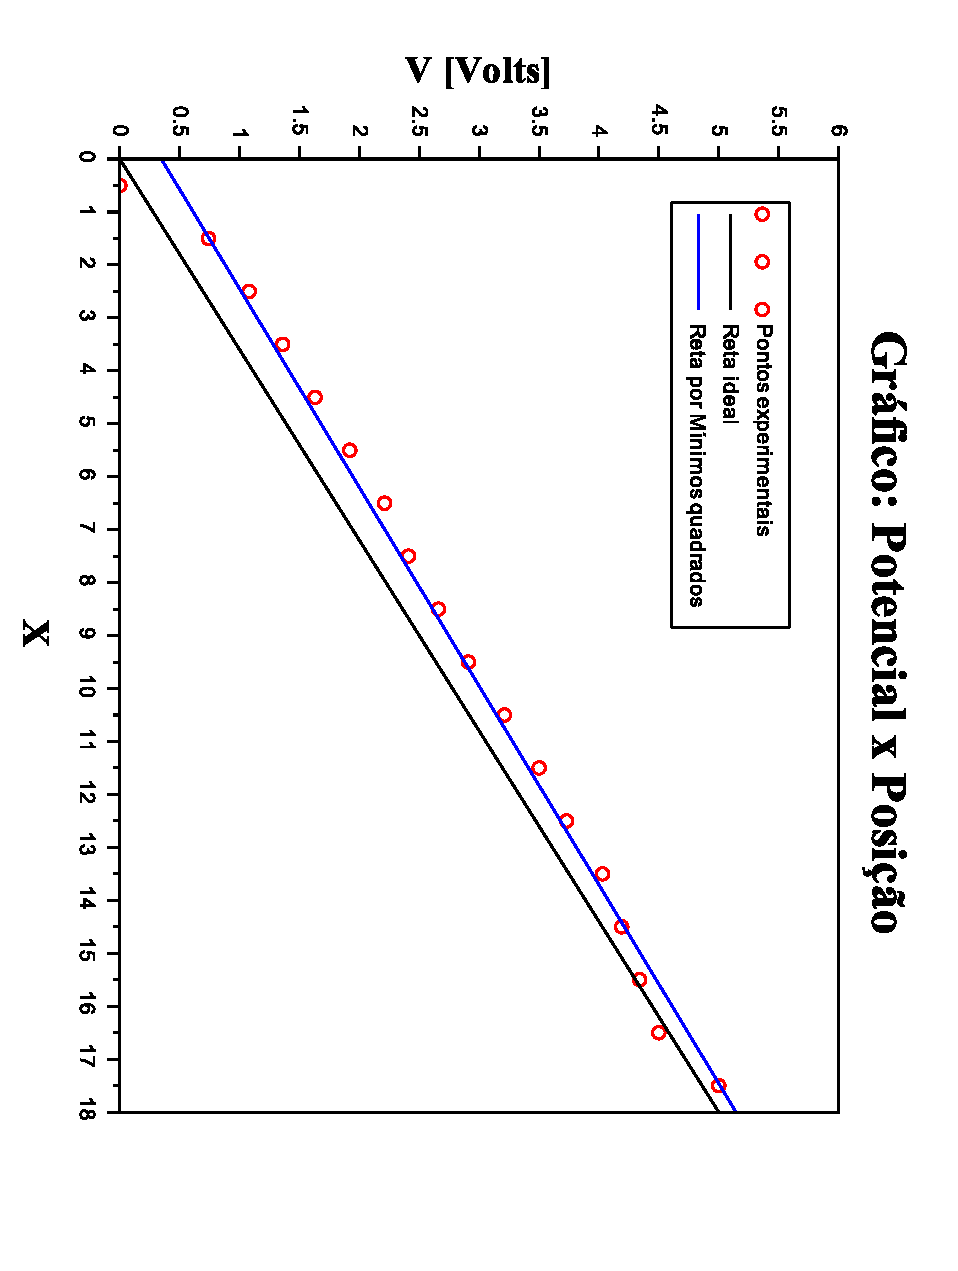
\includegraphics[scale=0.35,angle=90]{Figuras/Graph_18_points.pdf}
	\caption{Potencial em função da posição da trilha 1}
	\label{fig1}
\end{figure}


\begin{figure}[htb]
	\centering
		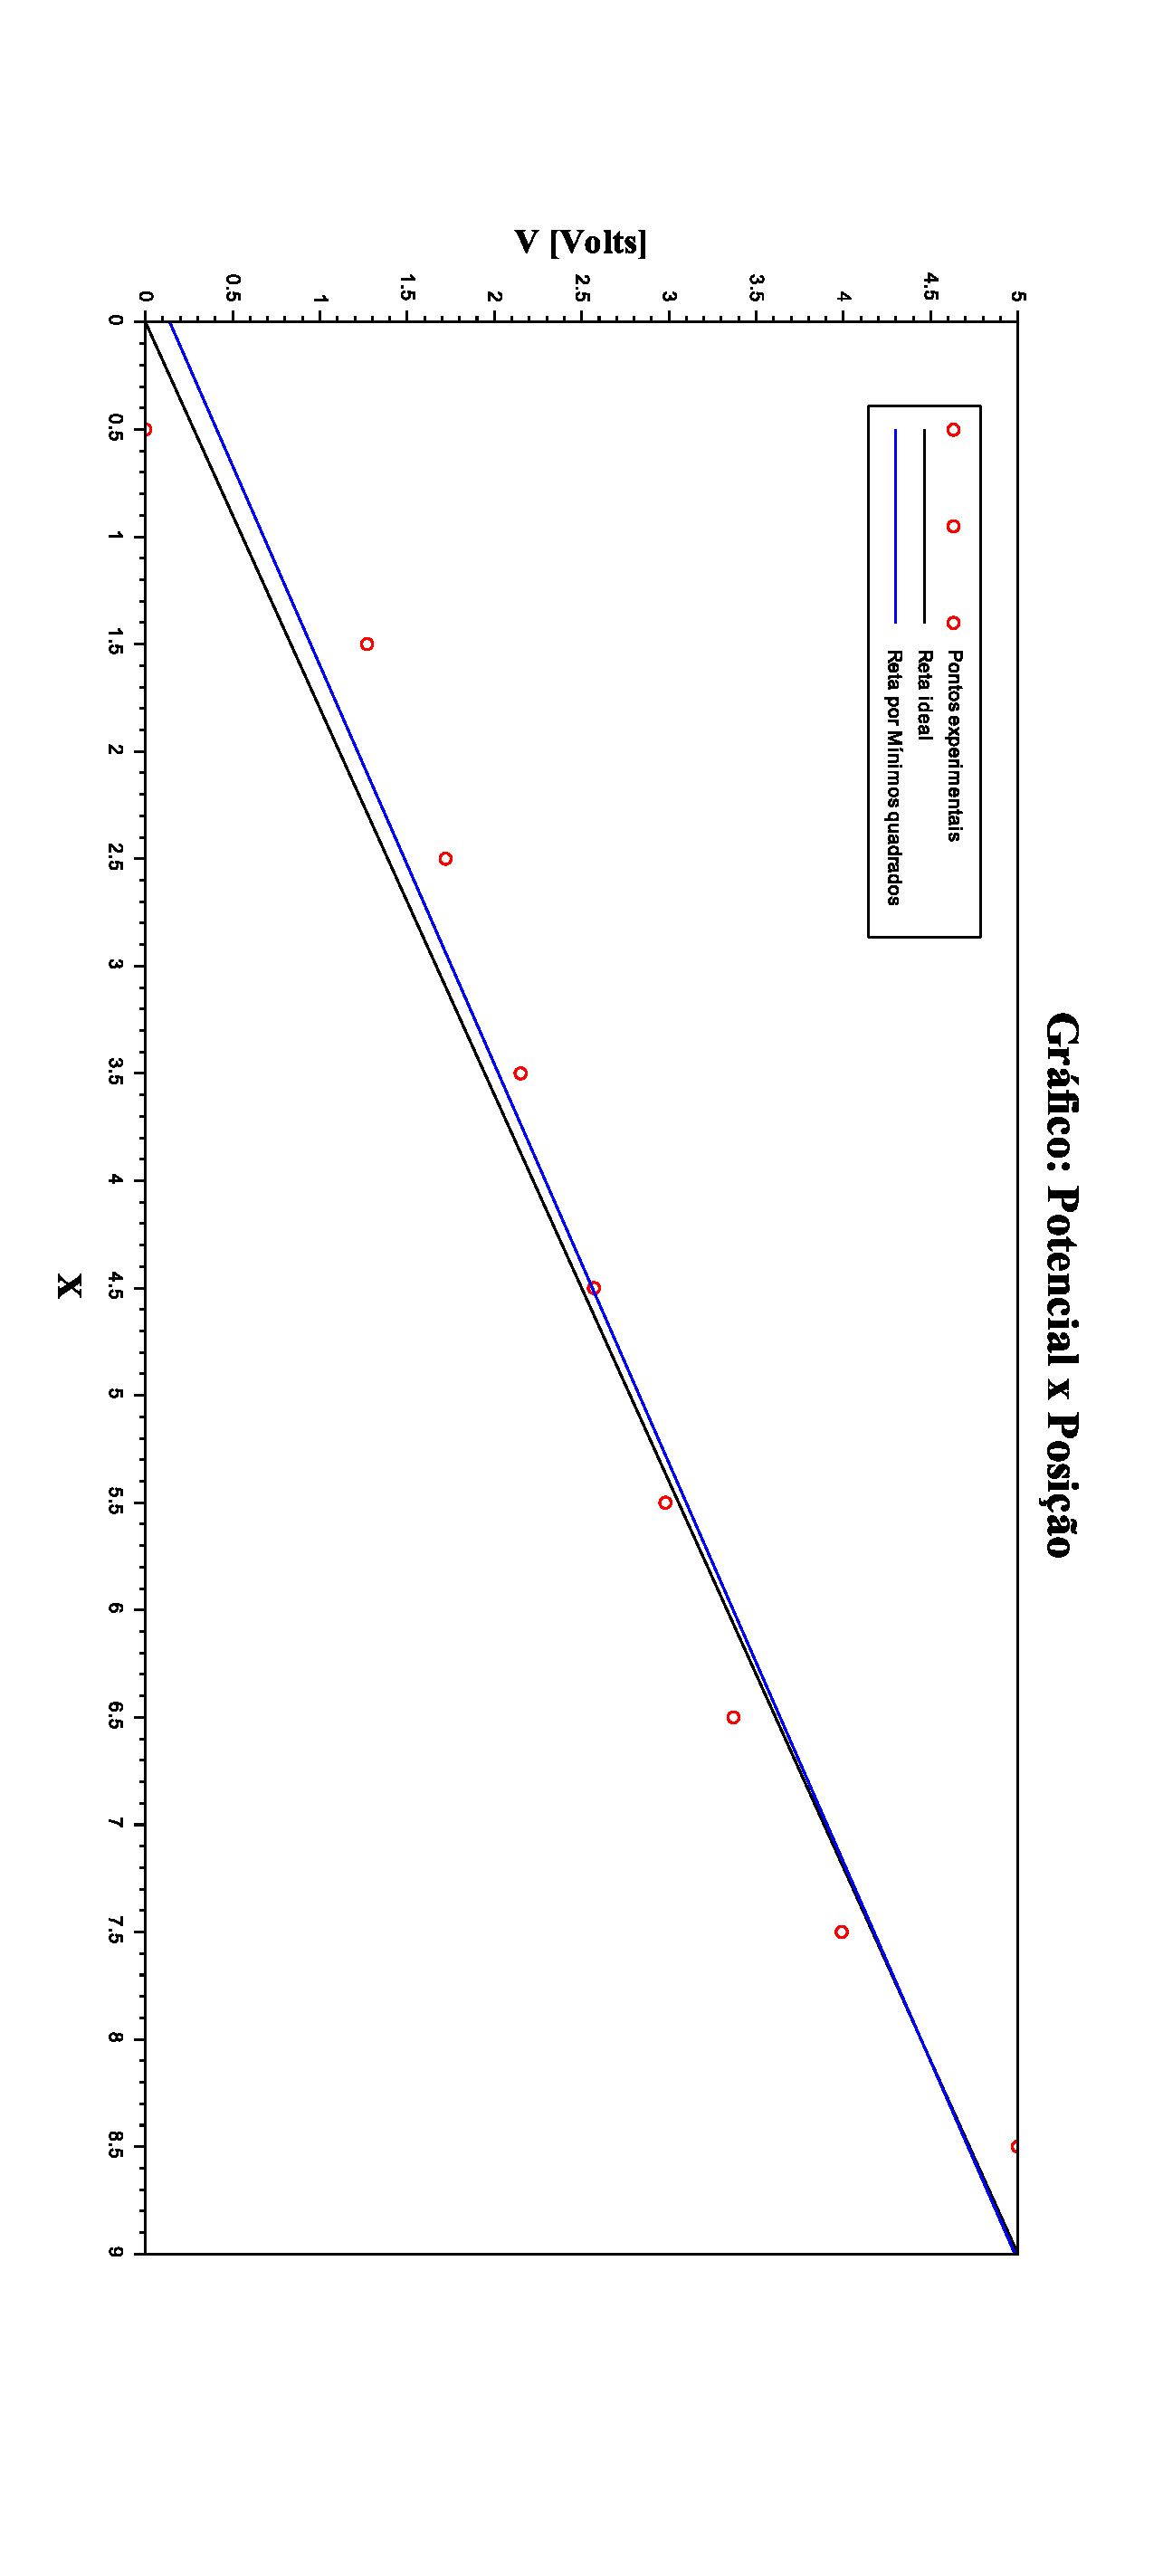
\includegraphics[width=.21\textwidth,angle=90]{Figuras/Graph_9_points.pdf}
		%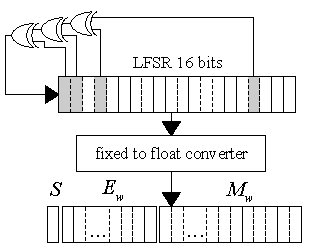
\includegraphics[scale=0.9]{figures/fig1_RNG.eps}
	\caption{Potencial em função da posição da trilha 2}
	\label{fig2}
\end{figure}

O gráfico da resistência pela posição $(R\times X)$, construído a partir dos dados
da tabela experimental, permite concluir que a resistência elétrica R do resitor de grafite é diretamente proporcional a sua posição X, ou seja seu comprimento L, $$R \propto L$$.

A dispersão das medidas, apesar de serem muito pequenas não prejudicam a experimentação.
 E podem ser observadas mais facilmente no gráfico da trilha um, o que sugere um valor de dispersão maior. A dispersão reduz-se com o aumento da largura.
 
Outras característica podem ser consideradas importantes na definição deste valor. Entre elas estão a opacidade das trilhas de grafite, a direção em que a trilha foi desenhada e a relativa dificuldade em desenhar resistores com larguras e espessuras constantes e uniformes por toda a trilha. Também como os erros instrumentais da fonte de tensão e do multímetro utilizado. 

